\section{Auswertung}
\label{sec:Auswertung}
\subsection{Statische Messung}
\begin{figure}
	\centering
	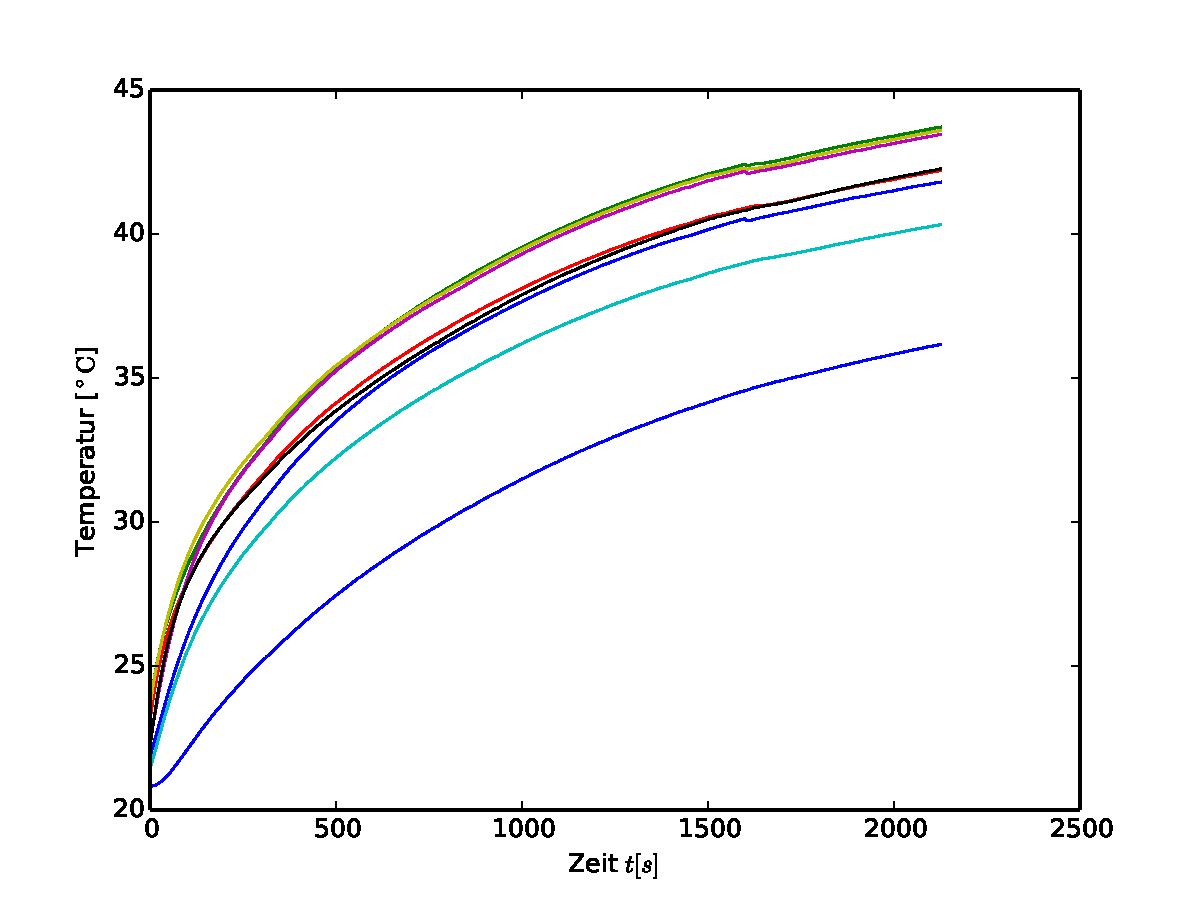
\includegraphics[width=0.7\textwidth]{Bilder/M1_Overview.pdf}
	\caption{Alle gemessenen Temperaturen ohne Beschriftung}
\end{figure}
Alle Temperaturverläufe werden in Diagramm \ref{fig:overview1} gleichzeitig aufgetragen. Es zeigt, dass der allgmeine Verlauf der Temperatur unabhängig von dem Material und der Entfernung des Messpunktes ist. Die Temperaturkurven zeigen jeweils beschränktes Wachstum und sind streng monoton wachsend.
\begin{figure}[p]
	\centering
	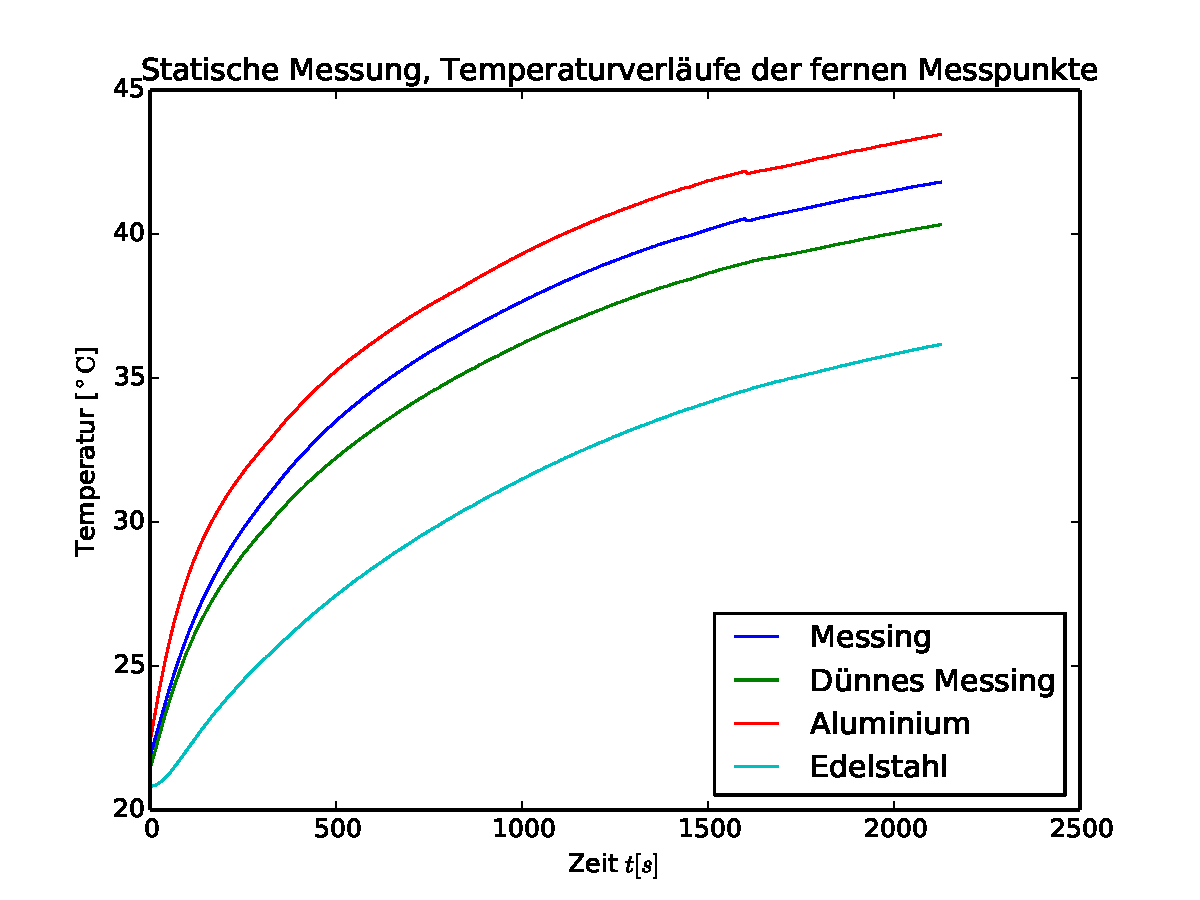
\includegraphics[width=0.8\textwidth]{Bilder/M1_Tempverl.pdf}
	\caption{Verlauf der Temperaturen an den entfernten Messpunkten.}
	\label{fig:entftemp}
\end{figure}
Im Diagramm \ref{fig:entftemp} wird der Temperaturverlauf bei den entfernten Messpunkten T1, T4, T5, T8 (vgl. Abbildung \ref{fig:platine}) gezeigt. 
Die Kurve von Aluminium hat zu Beginn des Experiments den stärksten Anstieg und liegt über den Kurven der anderen Metallstäbe. 
Beide Kurven der Messingstäbe haben vergleichbare Steigungen;
die Kurve des breiten Messingstabes liegt dabei über der des schmalen Stabes und hat am Endpunkt der Messung zu dieser eine Temperaturdifferenz von etwa $1 \si{\degreeCelsius}$. 
Die Kurve von Edelstahl ist deutlich von den Kurven der anderen Metallstäbe entfernt und weist die geringste Steigung auf. 
Zum Endpunkt der Messung liegt zwischen den Messpunkten von Aluminium und Edelstahl eine maximale Temperaturdifferenz von etwa $7 \si{\degreeCelsius}$ vor. 

Zirka 700 Sekunden nach Beginn des Erwärmens liegen an den entfernten Messpunkten die Temperaturen nach Tabelle \ref{tab:700} vor. Die höchste Temperatur hat der Aluminiumstab, die geringste Temperatur weist Edelstahl auf.
\begin{table}
	\centering
	\begin{tabular}{cccc}
	\toprule
	{Edelstahl}&{Messing,dünn}&{Messing}&{Aluminium}\\
	\midrule
	29$\si{\degreeCelsius}$& 34$\si{\degreeCelsius}$& 35.4$\si{\degreeCelsius}$& 37$\si{\degreeCelsius}$\\
	\bottomrule
	\end{tabular}
	\caption{Temperaturen an entfernten Messpunkten bei $t=700\si{\second}$.}
	\label{tab:700}
\end{table}

Es wird sichtbar, dass bei gleicher Zeit durch den Aluminiumstab mehr Wärme geleitet wird als durch die Messingstäbe und durch den Edelstahlstab. 
Aluminium hat demnach die größte Wärmeleitfähigkeit.

Mit Gleichung \eqref{waermemenge} kann der Wärmestrom $\frac{\Delta{Q}}{\Delta{t}}$ innerhalb der Stäbe bestimmt werden. 
Dabei ist $\kappa$ der Litearaturwert der Wärmeleitfähigkeit des betrachteten Metalls und $A$ die Querschnittsfläche (vgl. hierzu \cite{V204}) des jeweiligen Stabes.
$\frac{\partial T}{\partial x}$ ist der Temperaturgradient innerhalb des Stabes und wird hier mit $\frac{\Delta T}{\Delta x}$ und $\Delta x \approx 0.03\si{\meter}$ beschrieben.
Es ergibt sich die Wärmemenge $\mathup{d}Q$ zu fünf unterschiedlichen Zeiten.
\begin{table}
	\centering
	\begin{tabular}{cccccc}
	\sisetup{table-format=1.4}\\
\toprule
	Stab & $50\:\si\second$ & $500\:\si\second$ & $1000\:\si\second$ & $1500\:\si\second$ & $2000\:\si\second$ \\
	\midrule
	Messing 1 &$-0.4973\:\si{\watt}$ &$-0.3552\:\si{\watt}$&$-0.3629\:\si{\watt}$&$-0.3725\:\si{\watt}$&$-0.3648\:\si{\watt}$\\
	Messing 2 &$-0.2867\:\si{\watt}$& $-0.2128\:\si{\watt}$&$-0.2150\:\si{\watt}$&$-0.2173\:\si{\watt}$&$-0.2106\:\si{\watt}$\\
	Aluminium &$-0.4174\:\si{\watt}$&$-0.0677\:\si{\watt}$&$-0.0564\:\si{\watt}$&$-0.0564\:\si{\watt}$&$-0.0489\:\si{\watt}$\\
	Edelstahl &$-0.1116\:\si{\watt}$&$-0.1538\:\si{\watt}$&$-0.1536\:\si{\watt}$&$-0.1524\:\si{\watt}$&$-0.1469\:\si{\watt}$\\
	\bottomrule
	\end{tabular}
	\caption{Wärmemengen d$Q$ der Probenstäbe zu fünf unterschiedlichen Zeiten.}
	\label{tab:waememengen}
\end{table}

\begin{figure}
	\centering
	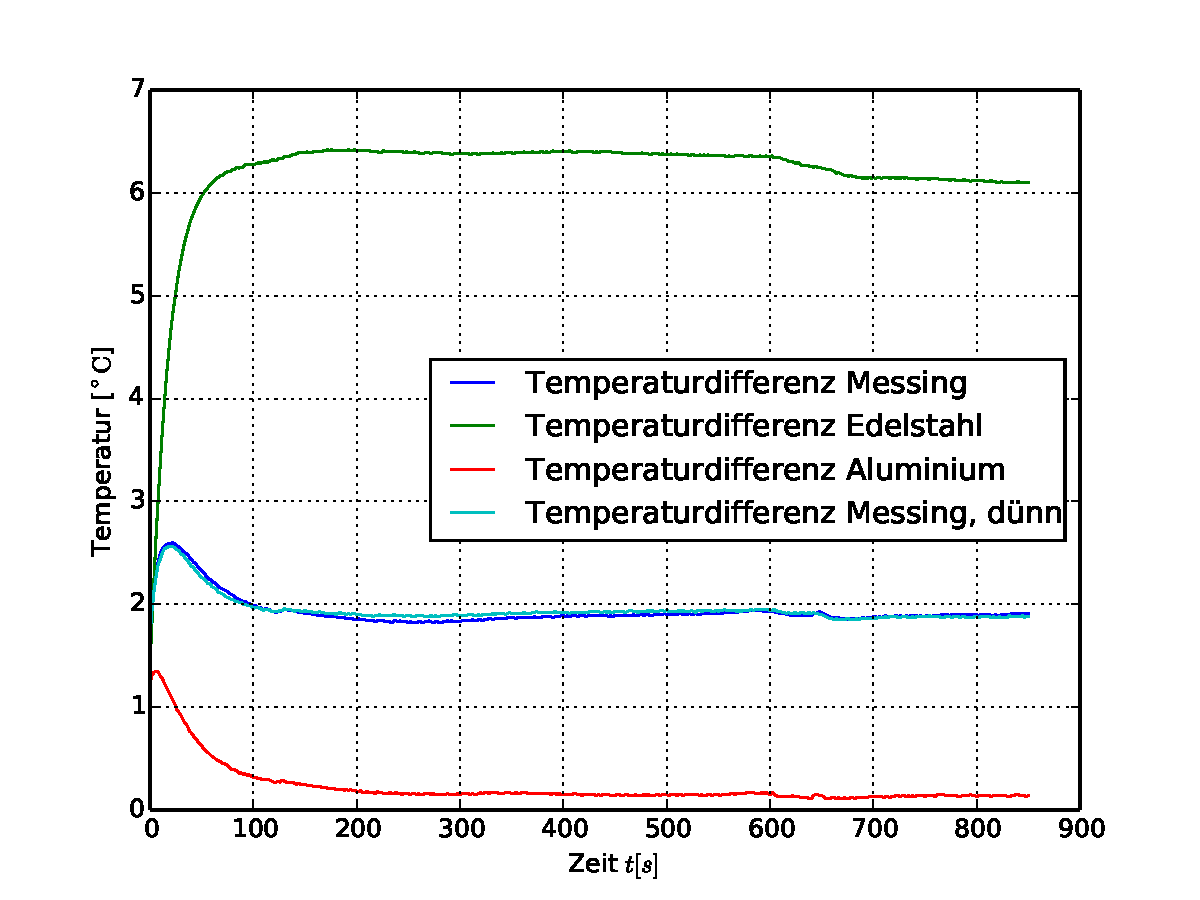
\includegraphics[width=0.8\textwidth]{Bilder/M1_Tempdiff.pdf}
	\caption{Temperaturdifferenz der Messpunkte von Messing und Edelstahl.}
	\label{fig:tempverl}
\end{figure}

Im Diagramm \ref{fig:tempverl} ist die Temperaturdifferenz innerhalb eines Stabes für den Edelstahl- und für den Messingstab aufgetragen. 
Es wird deutlich, dass die Differenzkurve für Edelstahl näherungsweise ein beschränktes Wachstum beschreibt und kurz nach Beginn der Erwärmung einen Grenzwert erreicht, der bei etwa  $6.25 \si{\degreeCelsius}$ liegt.
Die Differenzkurve des Messingstabes steigt zu Beginn der Messung an und erreicht kurz nach Beginn mit $2.6 \si{\degreeCelsius}$ ihr globales Maximum. 
Nach dem Maximum nimmt die Differenz exponentiell ab und erreicht einen Grenzwert von etwa $2 \si{\degreeCelsius}$.
Der Vergleich der Kurven zeigt, dass der Messingstab gegenüber dem Edelstahlstab den Grenzwert der Temperaturdifferenz schneller erreicht.

\subsection{Dynamische Messung bei 80 Sekunden-Periode}
Die Diagramme \ref{fig:M2Messing} und \ref{fig:M2Alu} zeigen bei periodischer Anregung einer Temperaturwelle mit einer Periodendauer von 80 Sekunden den Temperaturverlauf an den jeweiligen Enden. 
Zusätzlich zum Verlauf sind sowohl die Extrema, als auch deren Amplitudenfunktion eingezeichnet. 
Die Messwerte ab dem neunten lokalen Maximum werden von der Auswertung aufgrund offensichtlicher Abweichungen ausgeschlossen.

Durch Eichung des Temperaturverlaufs mit eingezeichneter Amplitudenfunktion durch bilden der Differenz zwischen Temperaturverlauf und Amplitudenfunktion, ergeben sich nahezu gleichmäßige Schwingungen, die in Diagramm \ref{fig:M2MessingNorm} und \ref{fig:M2AluNorm} sichtbar sind. 
Diese werden im Folgenden als Grundschwingungen der Temperatur bezeichnet. 
In diesen Diagrammen ist zu erkennen, dass sich für eine gleichmäßige Schwingung jeweils die oberen Amplitudenfunktionen zum Eichen eignen.
\begin{figure}[h!]
	\centering
	\begin{subfigure}{0.9\textwidth}
	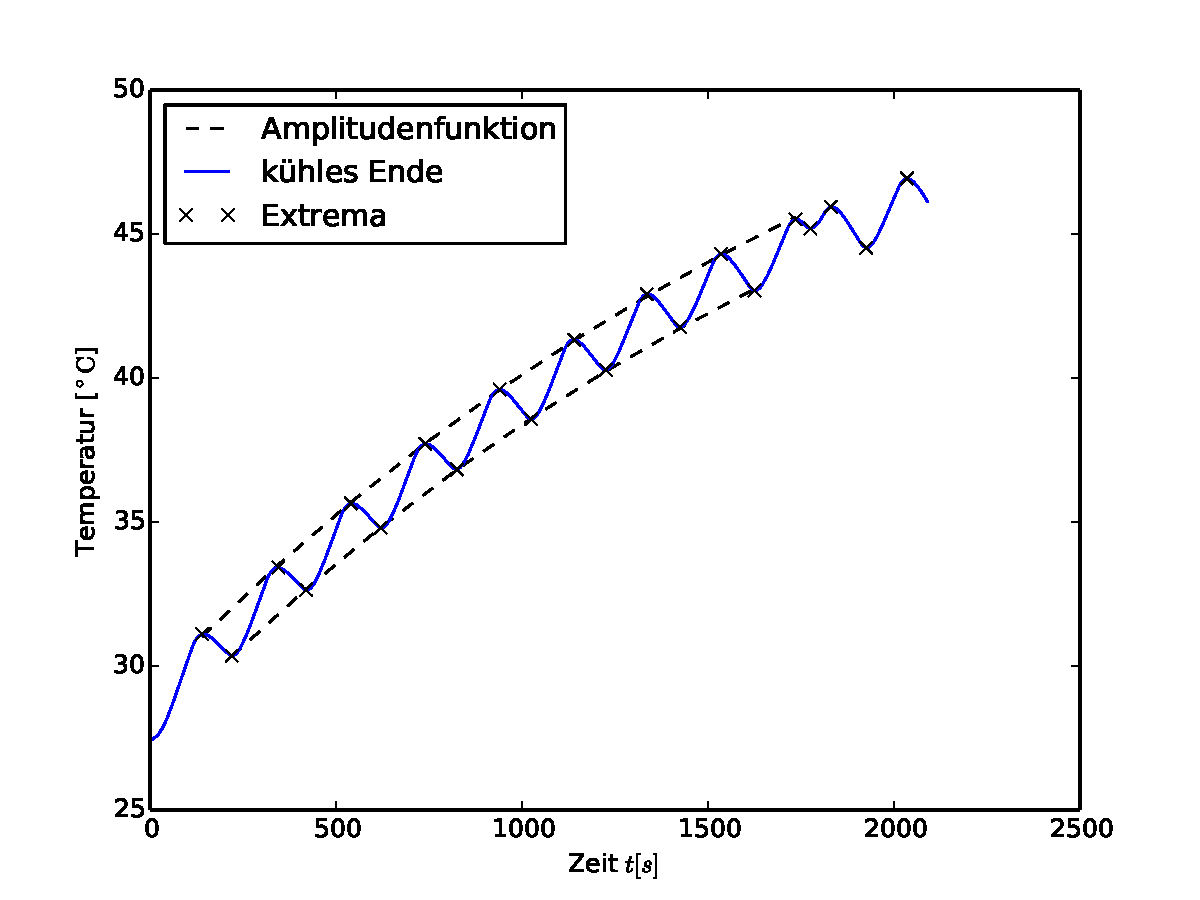
\includegraphics[width=\textwidth]{Bilder/M2_Messing_kuehl.pdf}
	\end{subfigure}
	\begin{subfigure}{0.9\textwidth}
	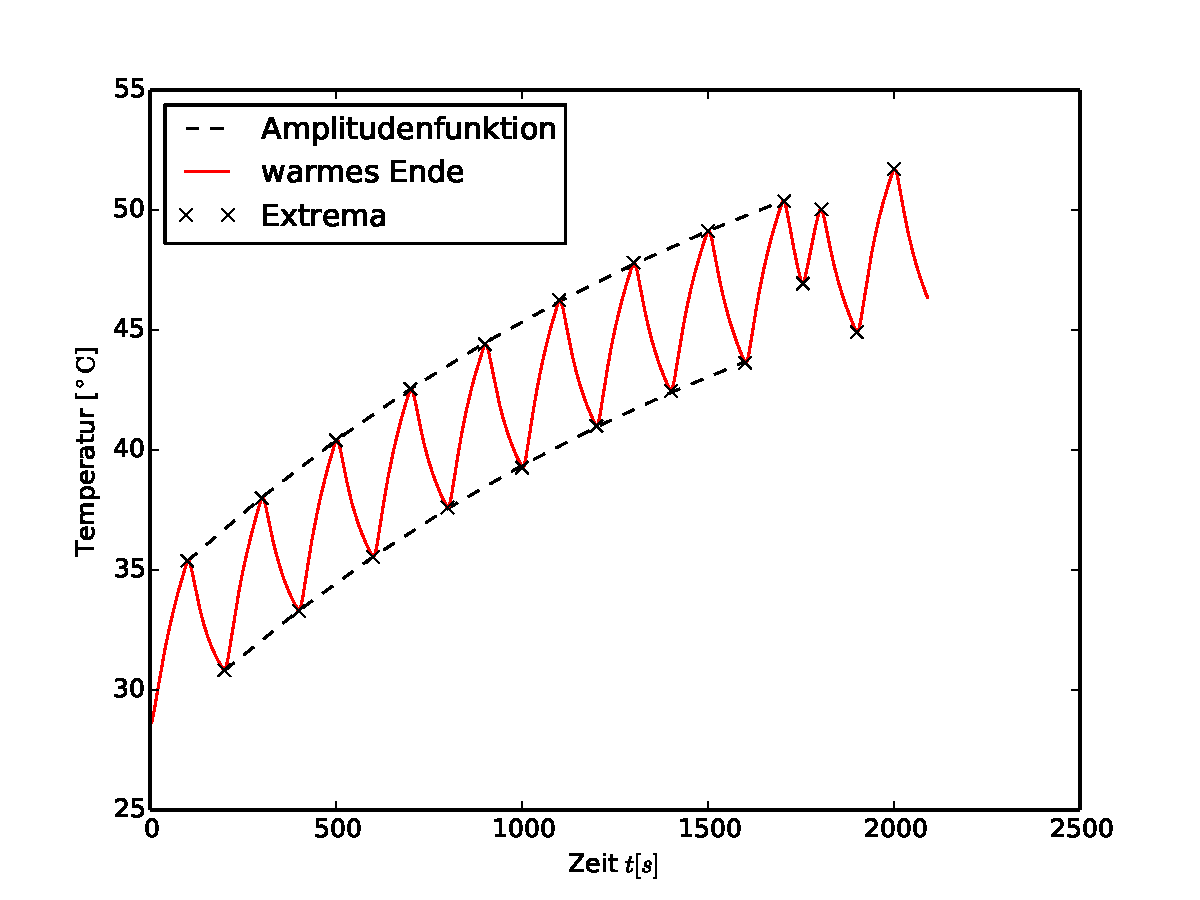
\includegraphics[width=\textwidth]{Bilder/M2_Messing_warm.pdf}
	\end{subfigure}
	\caption{Periodische Messung bei Messing mit 80 Sekunden-Periode}
	\label{fig:M2Messing}
\end{figure}
\begin{figure}[h!]
	\centering
	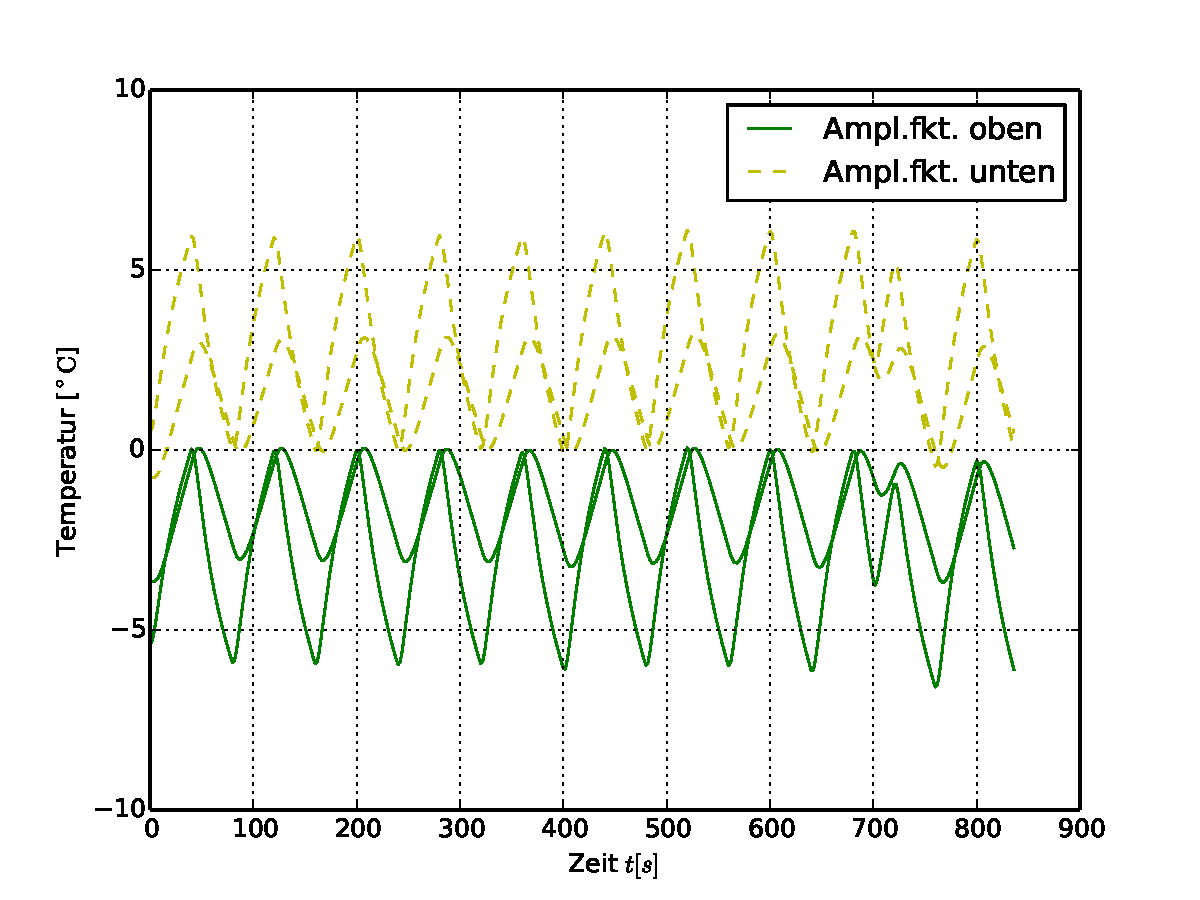
\includegraphics[width=0.8\textwidth]{Bilder/Normierungsauswahl/M2_Alu_norm.pdf}
	\caption{Normierung von Diagramm \ref{fig:M2Messing} auf Grundschwingung}
	\label{fig:M2MessingNorm}
\end{figure}
\begin{figure}[h!]
	\centering
	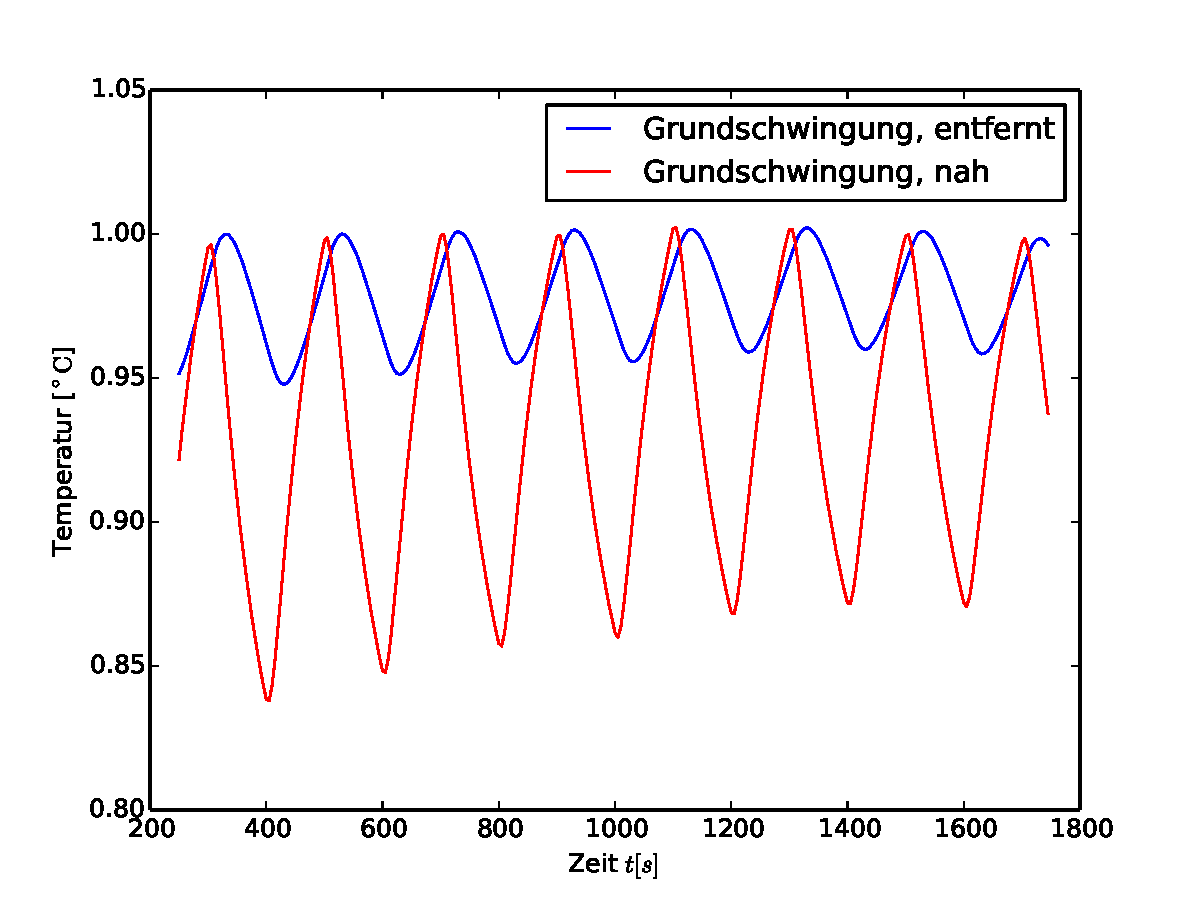
\includegraphics[width=0.7\textwidth]{Bilder/M2_Messing_norm.pdf}
	\caption{Ausgewählter Teil der Grundschwingung von Messing bei 80 Sekunden-Periode}
	\label{fig:M2MessingNormkurve}
\end{figure}
\begin{figure}[h!]
	\centering
	\begin{subfigure}{0.9\textwidth}
	\centering
	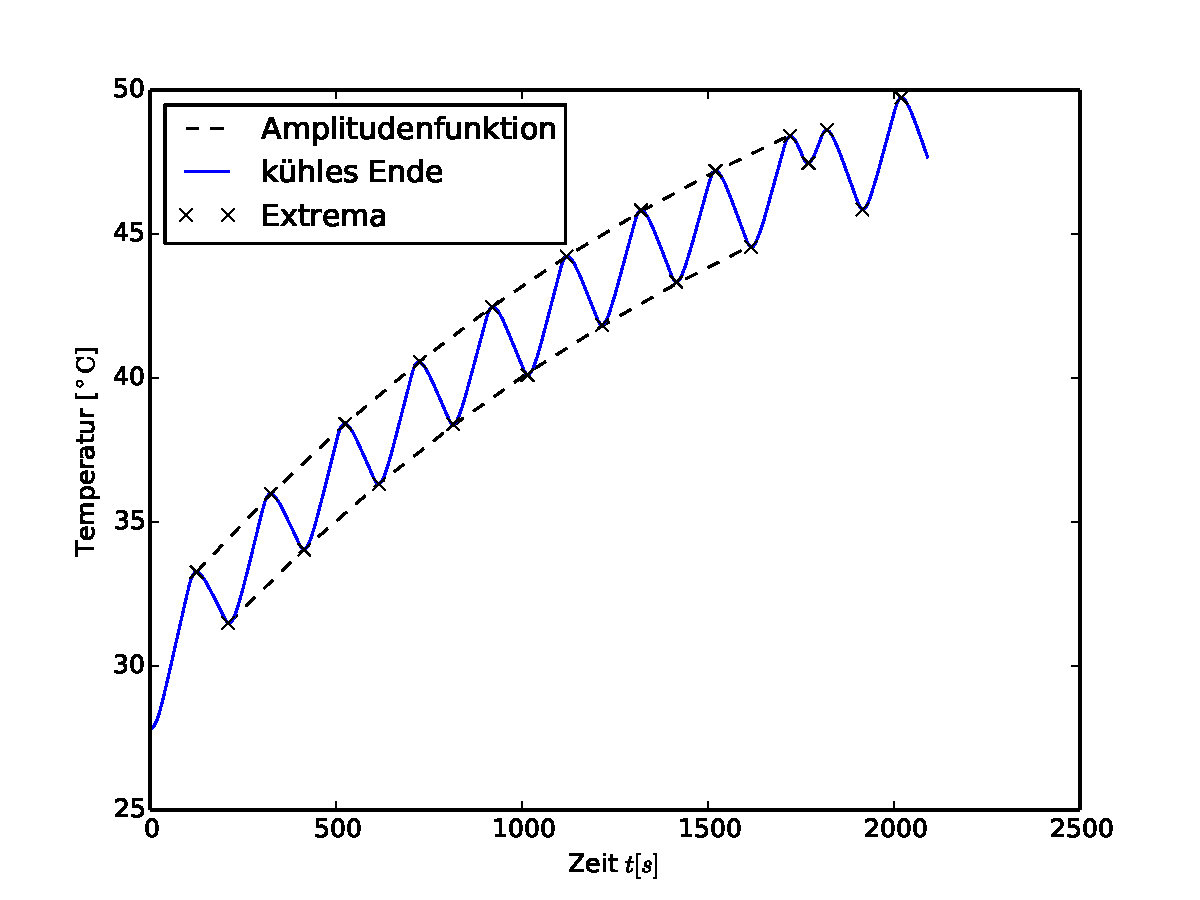
\includegraphics[width=\textwidth]{Bilder/M2_Alu_kuehl.pdf}
	\end{subfigure}
	\begin{subfigure}{0.9\textwidth}
	\centering
	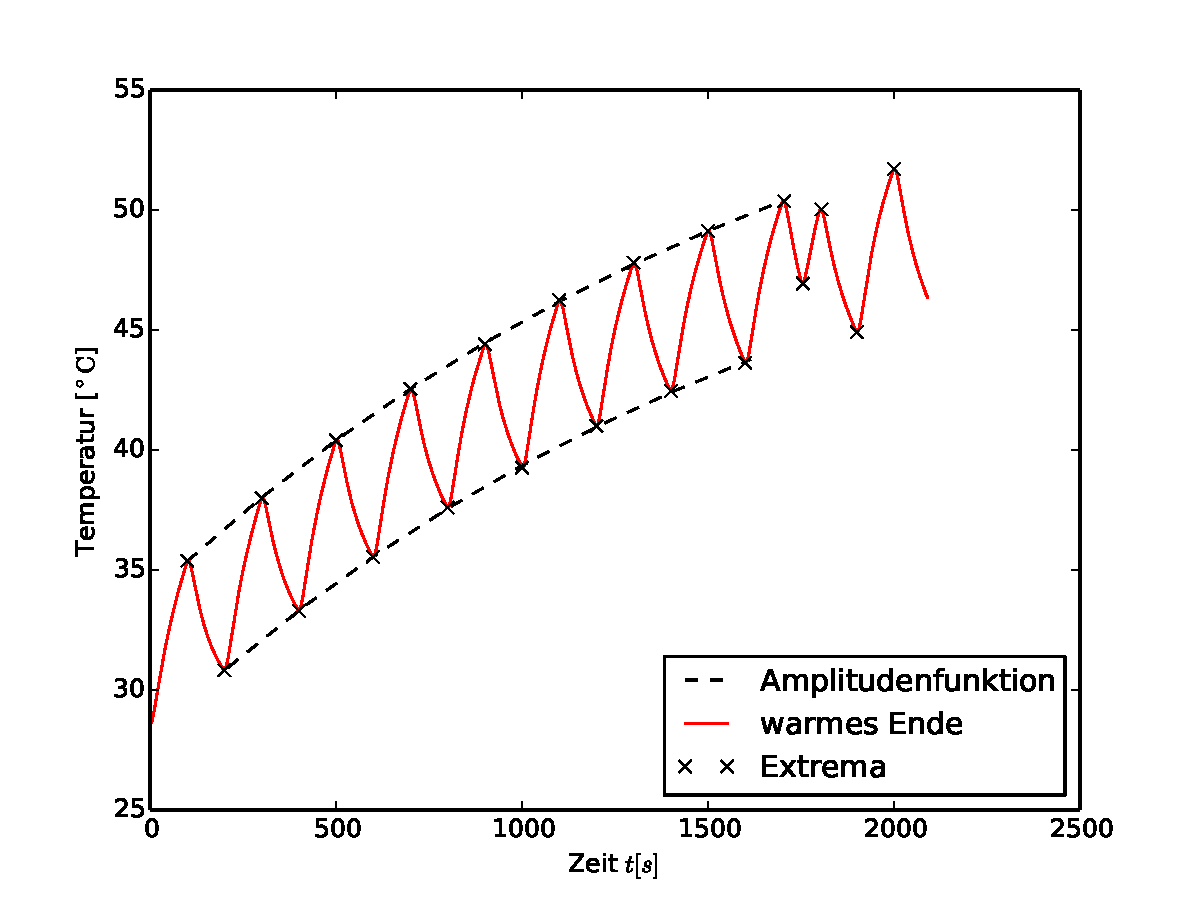
\includegraphics[width=\textwidth]{Bilder/M2_Alu_warm.pdf}
	\end{subfigure}
	\caption{Periodische Messung bei Aluminium mit 80 Sekunden-Periode.}
	\label{fig:M2Alu}
\end{figure}
\begin{figure}[h!]
	\centering
	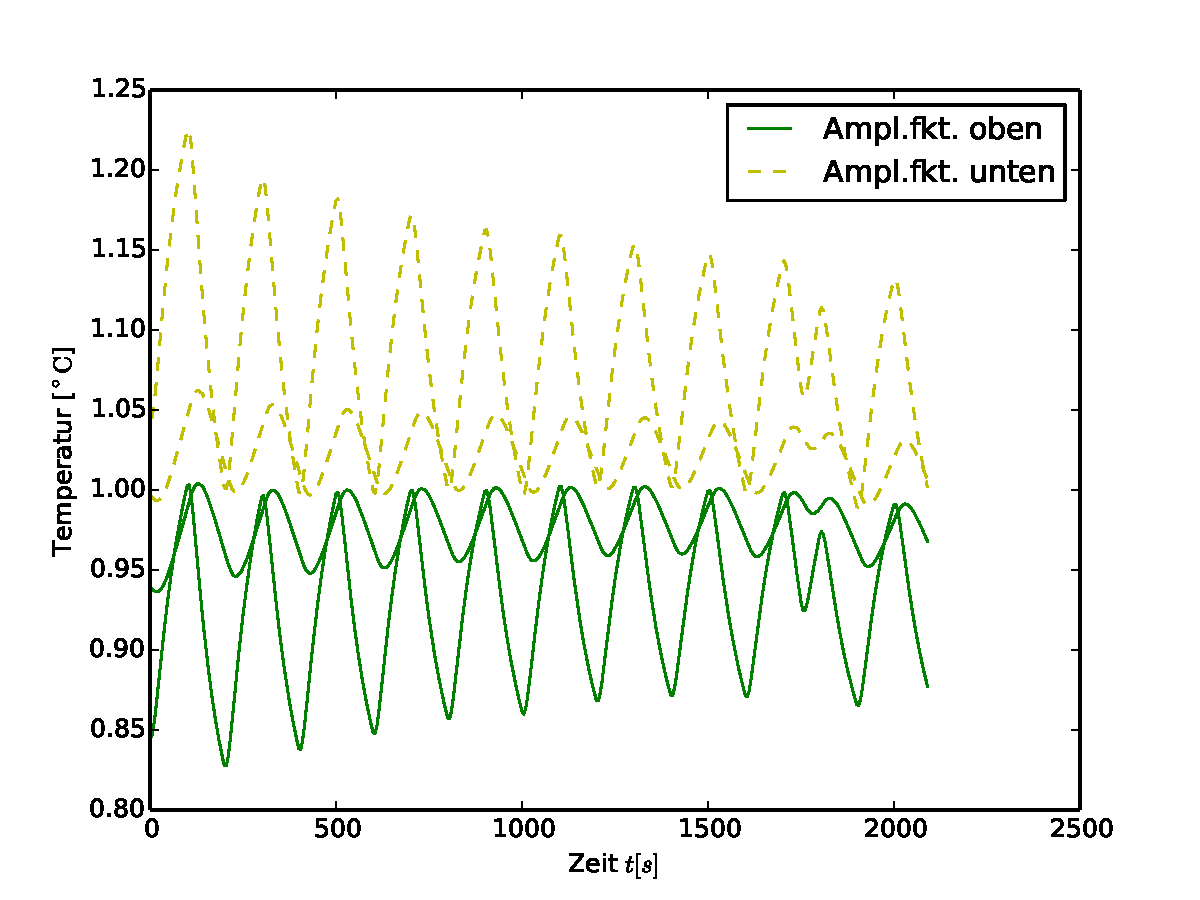
\includegraphics[width=0.8\textwidth]{Bilder/Normierungsauswahl/M2_Messing_norm.pdf}
	\caption{Normierung von Diagramm \ref{fig:M2Alu} auf Grundschwingung.}
	\label{fig:M2AluNorm}
\end{figure}
\begin{figure}[h!]
	\centering
	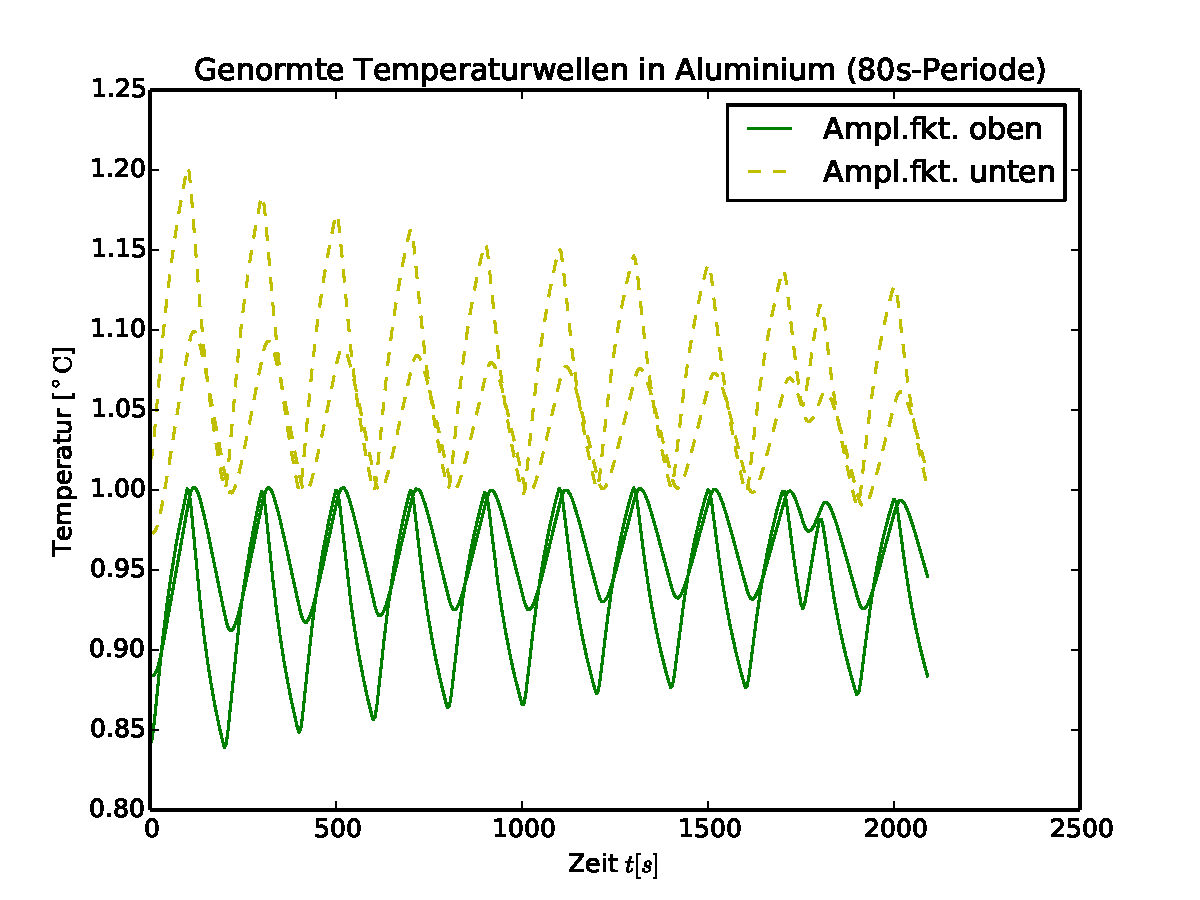
\includegraphics[width=0.7\textwidth]{Bilder/M2_Alu_norm.pdf}
	\caption{Ausgewählter Teil der Grundschwingung von Aluminium bei 80 Sekunden-Periode}
	\label{fig:M2AluNormkurve}
\end{figure}

\subsection{Dynamische Messung bei 200 Sekunden-Periode}
Für die Messung der Temperaturwellen bei einer Periodendauer von 200 Sekunden wird vollkommen analog vorgegangen.
Die Diagramme \ref{fig:M3Messing}, \ref{fig:M3Alu} und \ref{fig:M3Edelstahl} zeigen die Temperaturwellen der jeweiligen Metalle an den angegebenen Punkten. 
Zusätzlich zum Verlauf sind die Extrema markiert und deren Amplitudenfunktionen eingezeichnet.

Eicht man den Temperaturverlauf mit der eingezeichneten Amplitudenfunktionen, so ergeben sich die Grundschwingungen in den begleitenden Diagrammen \ref{fig:M3MessingNorm}, \ref{fig:M3AluNorm} und \ref{fig:M3Edelstahl}. 
Anhand dieser Diagramme wird ersichtlich, dass sich jeweils die oberen Amplitudenfunktionen dazu eignen, den Temperaturverlauf auf eine gleichmäßige Grundschwingung zu bringen.
\begin{figure}[h!]
	\centering
	\begin{subfigure}{0.9\textwidth}
	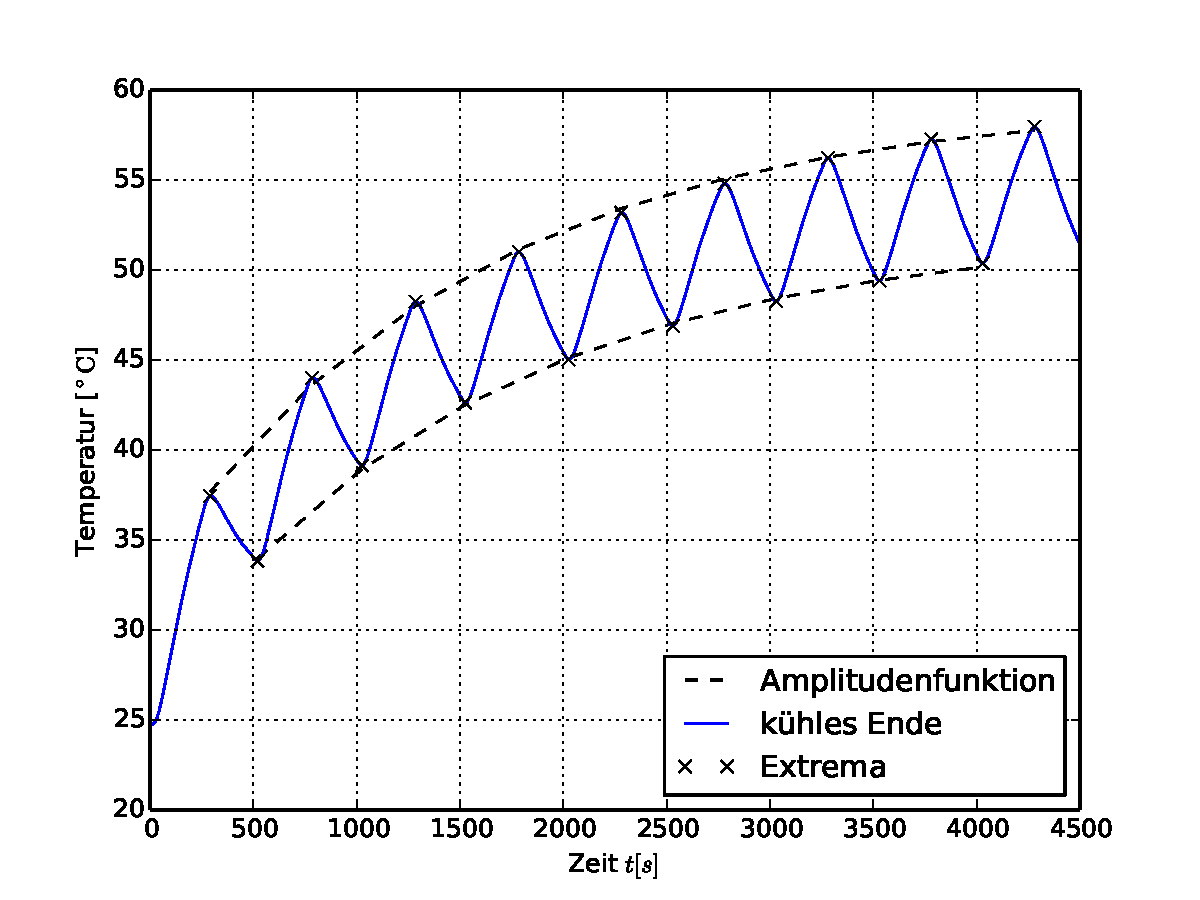
\includegraphics[width=\textwidth]{Bilder/M3_Messing_kuehl.pdf}
	\end{subfigure}
	\begin{subfigure}{0.9\textwidth}
	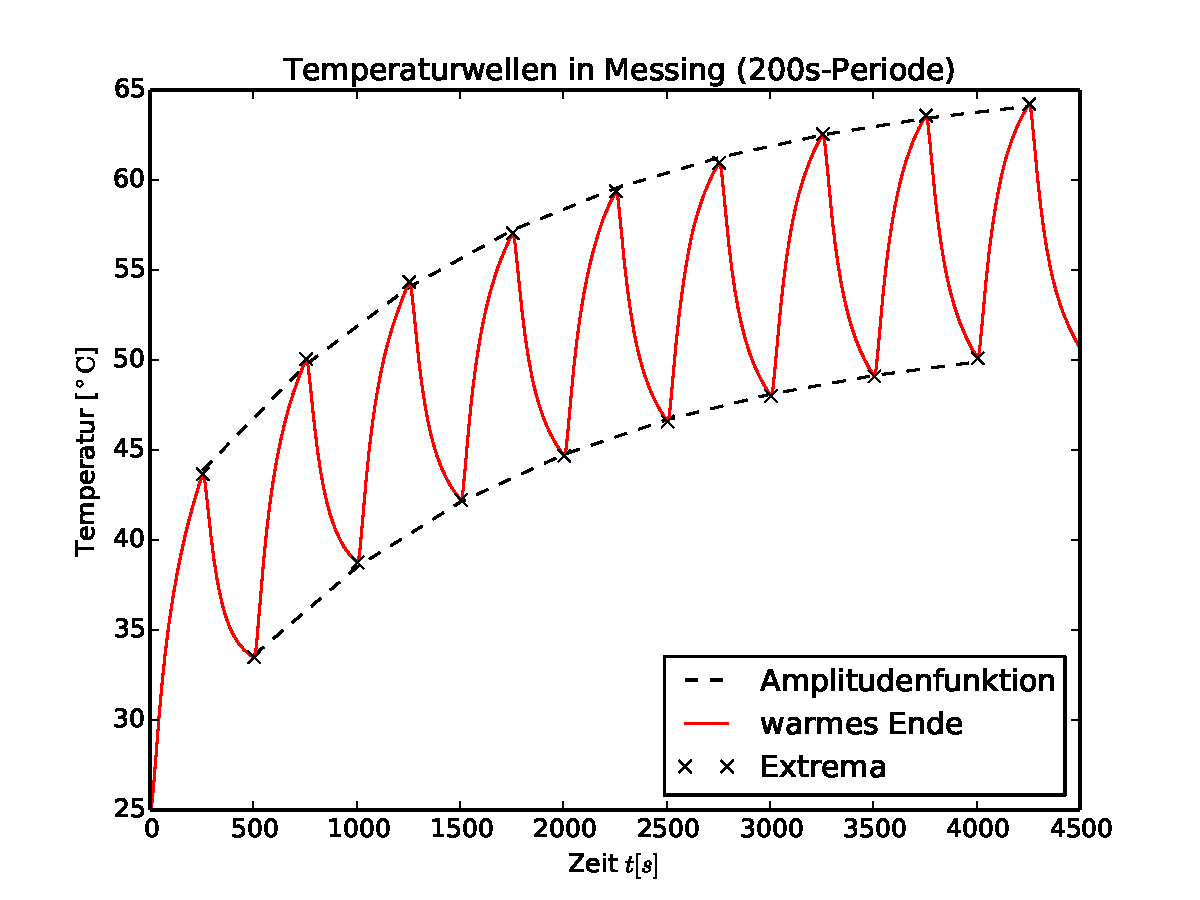
\includegraphics[width=\textwidth]{Bilder/M3_Messing_warm.pdf}
	\end{subfigure}
	\caption{Periodische Messung bei Messing mit 200 Sekunden-Periode.}
	\label{fig:M3Messing}
\end{figure}
\begin{figure}[h!]
	\centering
	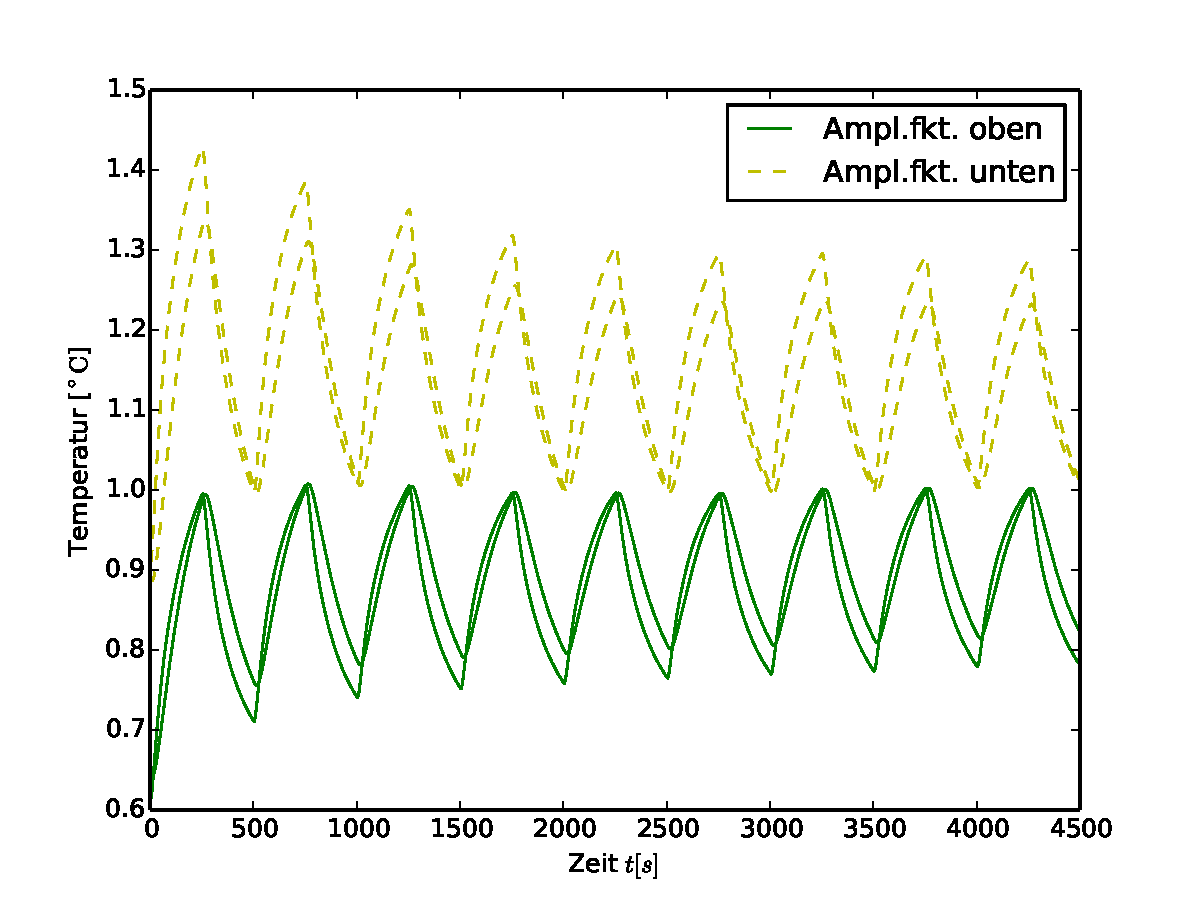
\includegraphics[width=0.8\textwidth]{Bilder/Normierungsauswahl/M3_Alu_norm.pdf}
	\caption{ Zwei Eich-Möglichkeiten von Diagramm \ref{fig:M3Messing} auf Grundschwingung}
	\label{fig:M3MessingNorm}
\end{figure}
\begin{figure}[h!]
	\centering
	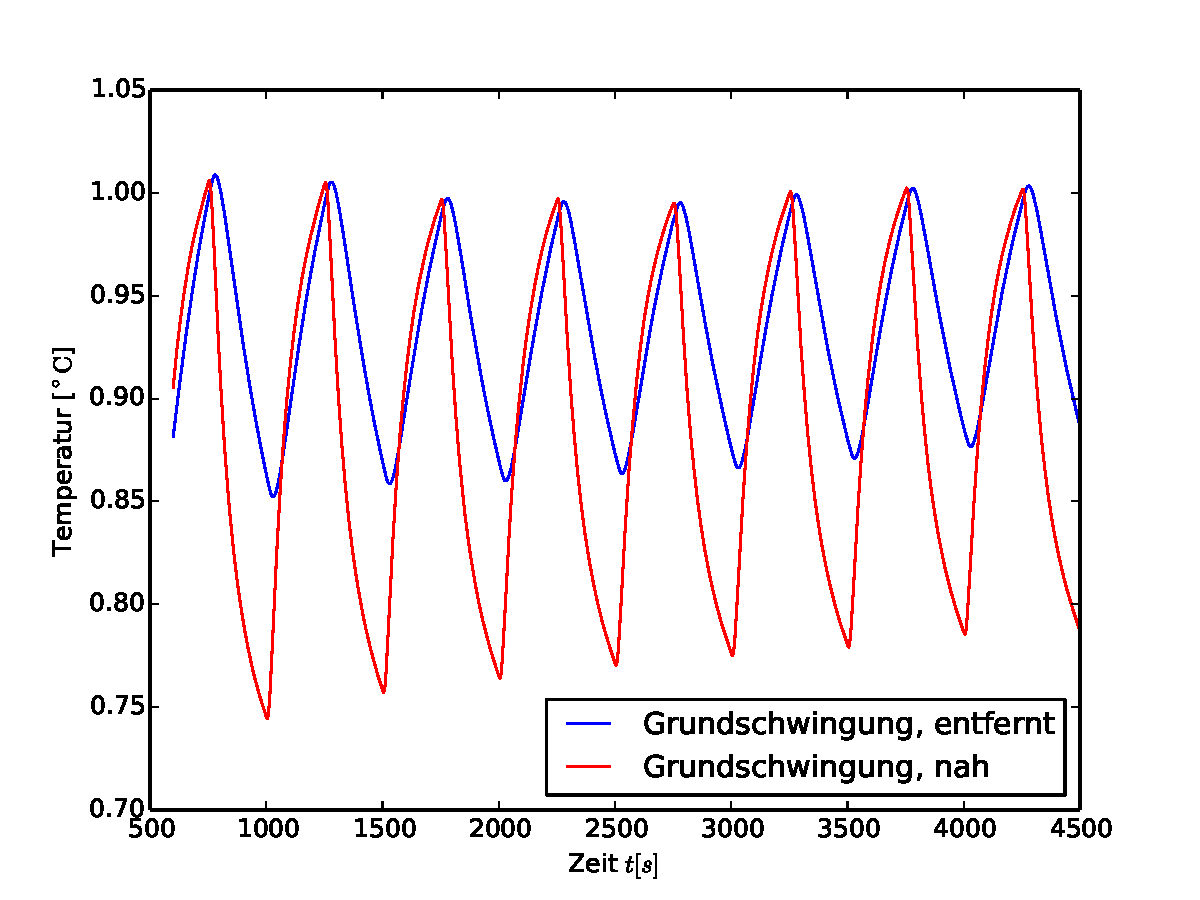
\includegraphics[width=0.7\textwidth]{Bilder/M3_Messing_norm.pdf}
	\caption{Ausgewählter Teil der Grundschwingung von Messing bei 200 Sekunden-Periode}
	\label{fig:M3MessingNormkurve}
\end{figure}
\begin{figure}[h!]
	\centering
	\begin{subfigure}{0.9\textwidth}
	\centering
	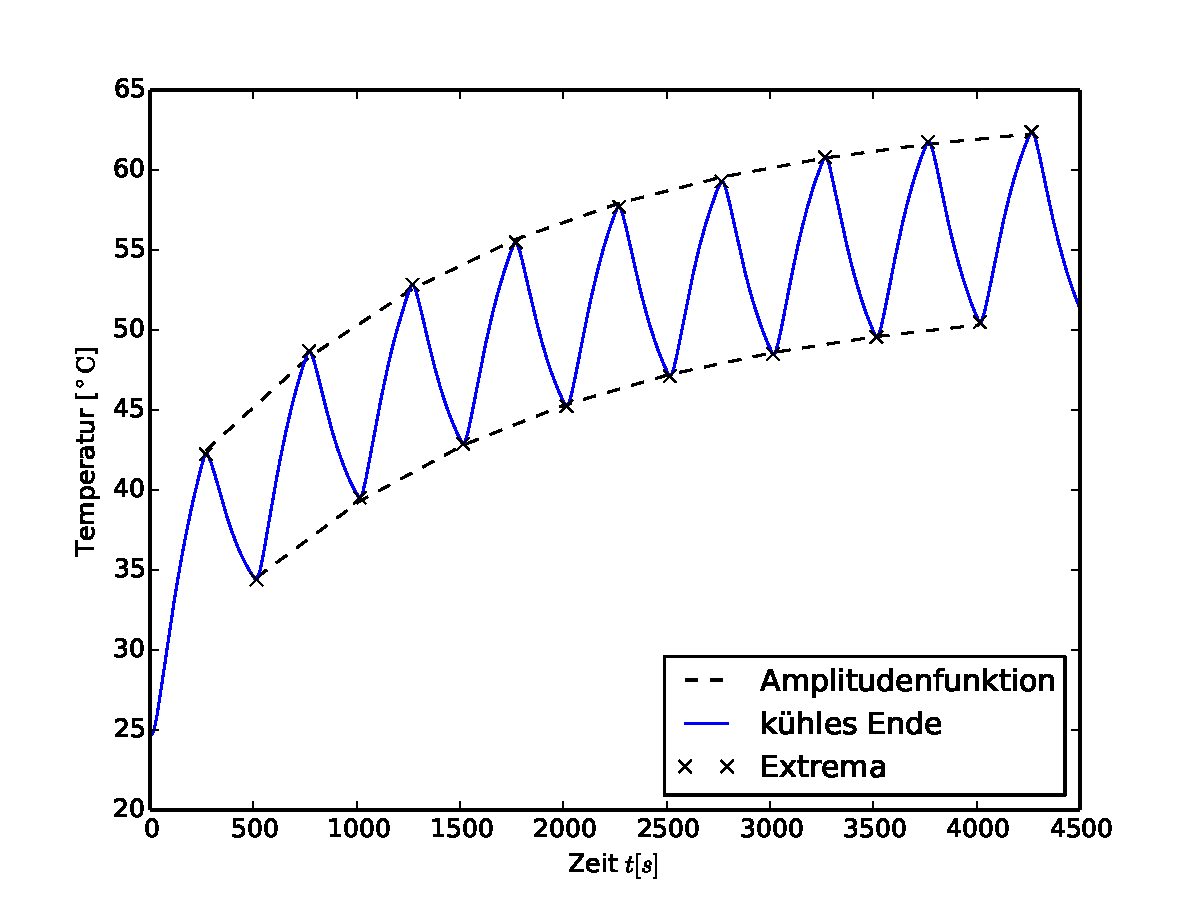
\includegraphics[width=\textwidth]{Bilder/M3_Alu_kuehl.pdf}
	\end{subfigure}
	\begin{subfigure}{0.9\textwidth}
	\centering
	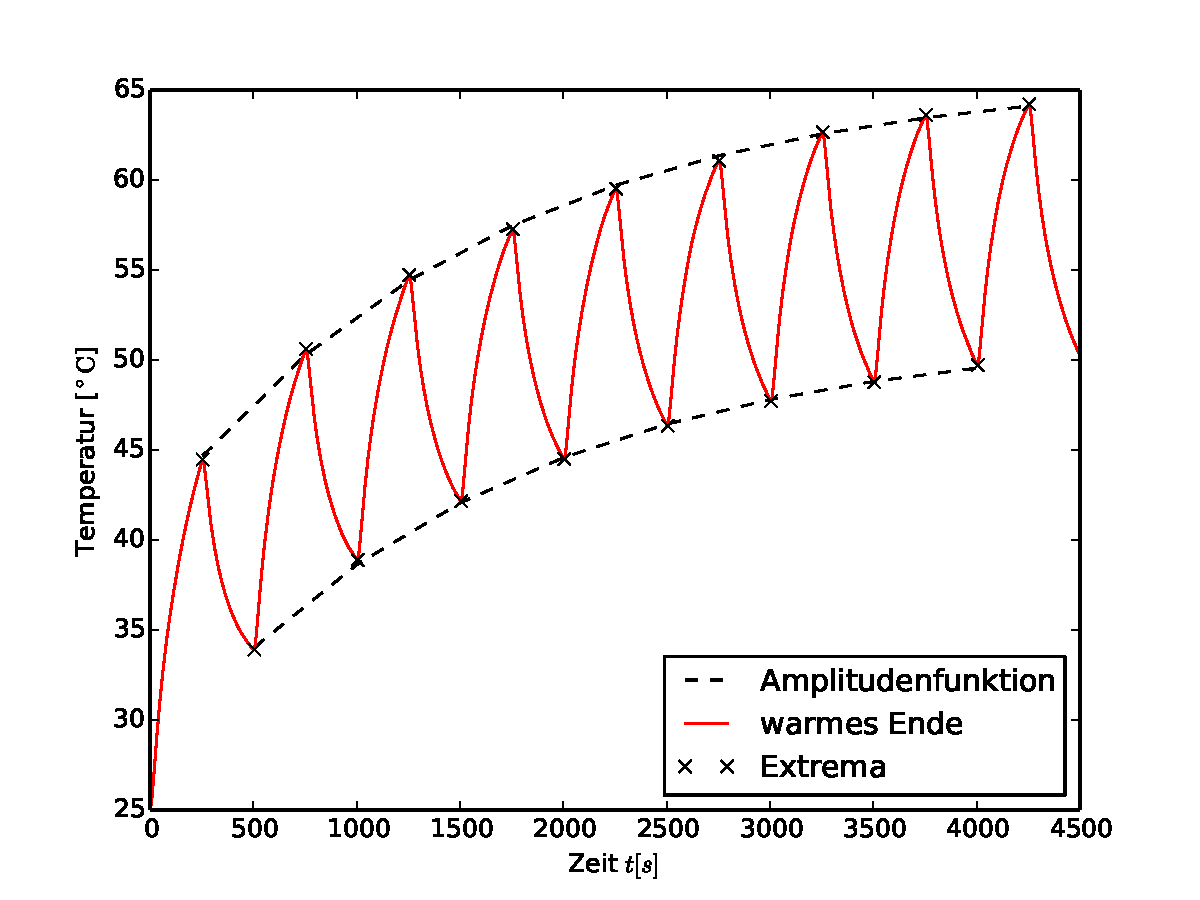
\includegraphics[width=\textwidth]{Bilder/M3_Alu_warm.pdf}
	\end{subfigure}
	\caption{Periodische Messung bei Aluminium mit 200 Sekunden-Periode.}
	\label{fig:M3Alu}
\end{figure}
\begin{figure}[h!]
	\centering
	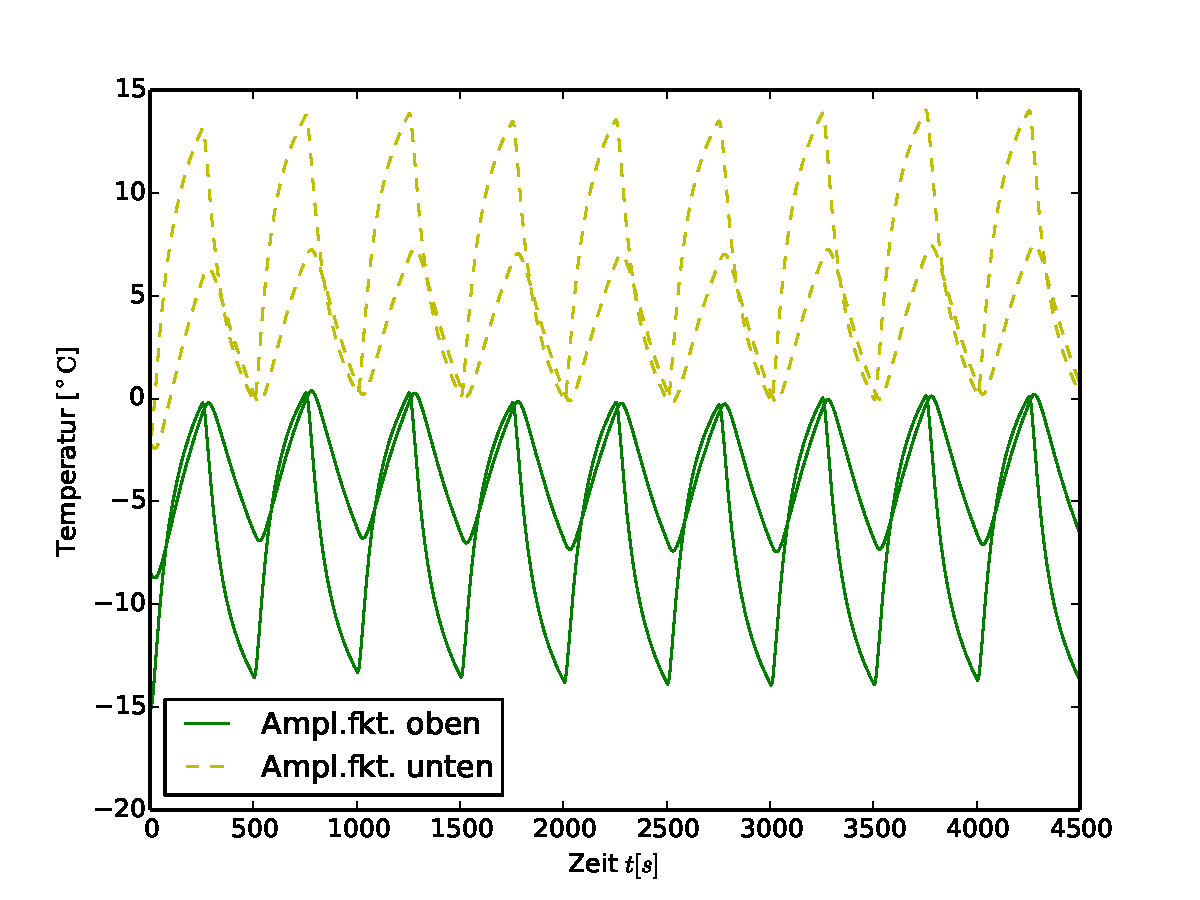
\includegraphics[width=0.8\textwidth]{Bilder/Normierungsauswahl/M3_Messing_norm.pdf}
	\caption{Zwei Eich-Möglichkeiten von Diagramm \ref{fig:M3Alu} auf Grundschwingung}
	\label{fig:M3AluNorm}
\end{figure}
\begin{figure}[h!]
	\centering
	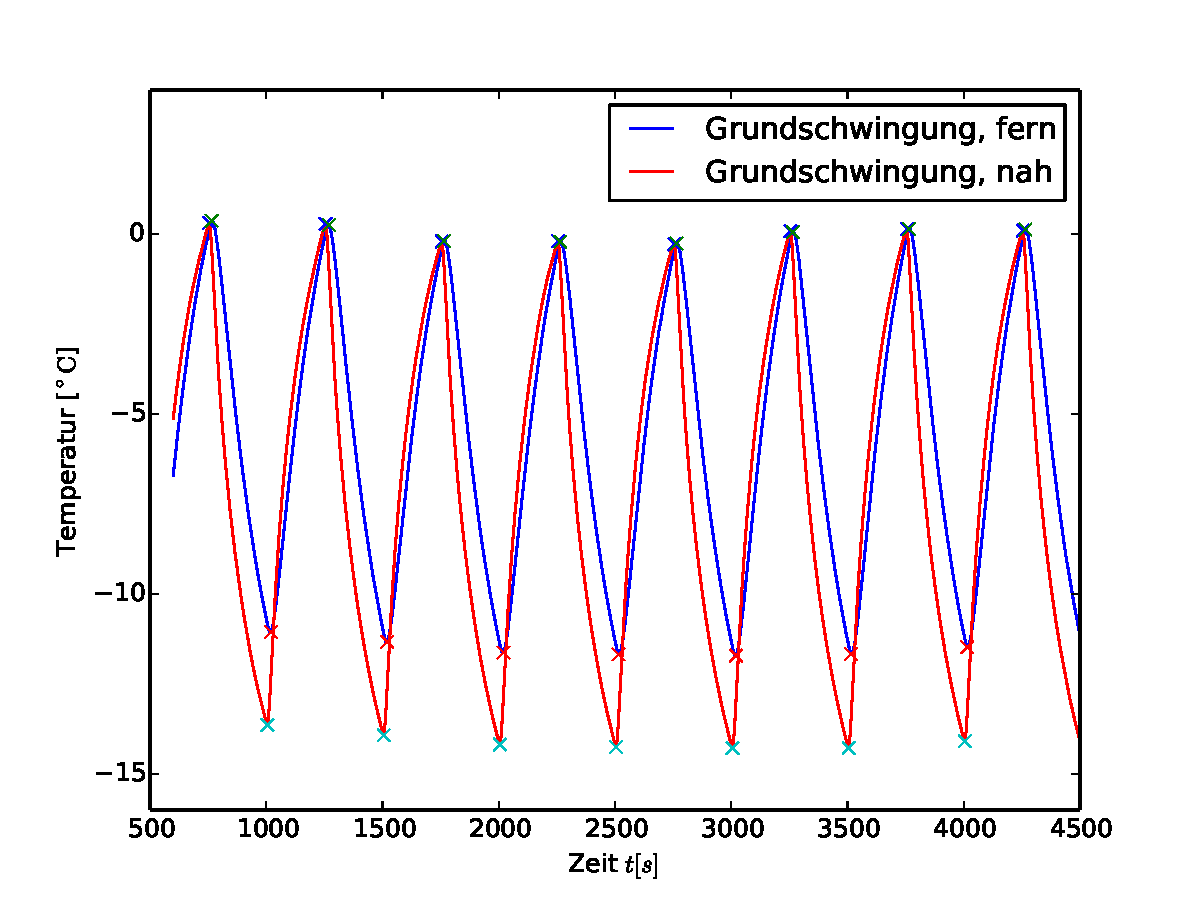
\includegraphics[width=0.7\textwidth]{Bilder/M3_Alu_norm.pdf}
	\caption{Ausgewählter Teil der Grundschwingung von Aluminium bei 200 Sekunden-Periode}
	\label{fig:M3AluNormkurve}
\end{figure}
\begin{figure}[h!]
	\centering
	\begin{subfigure}{0.9\textwidth}
	\centering
	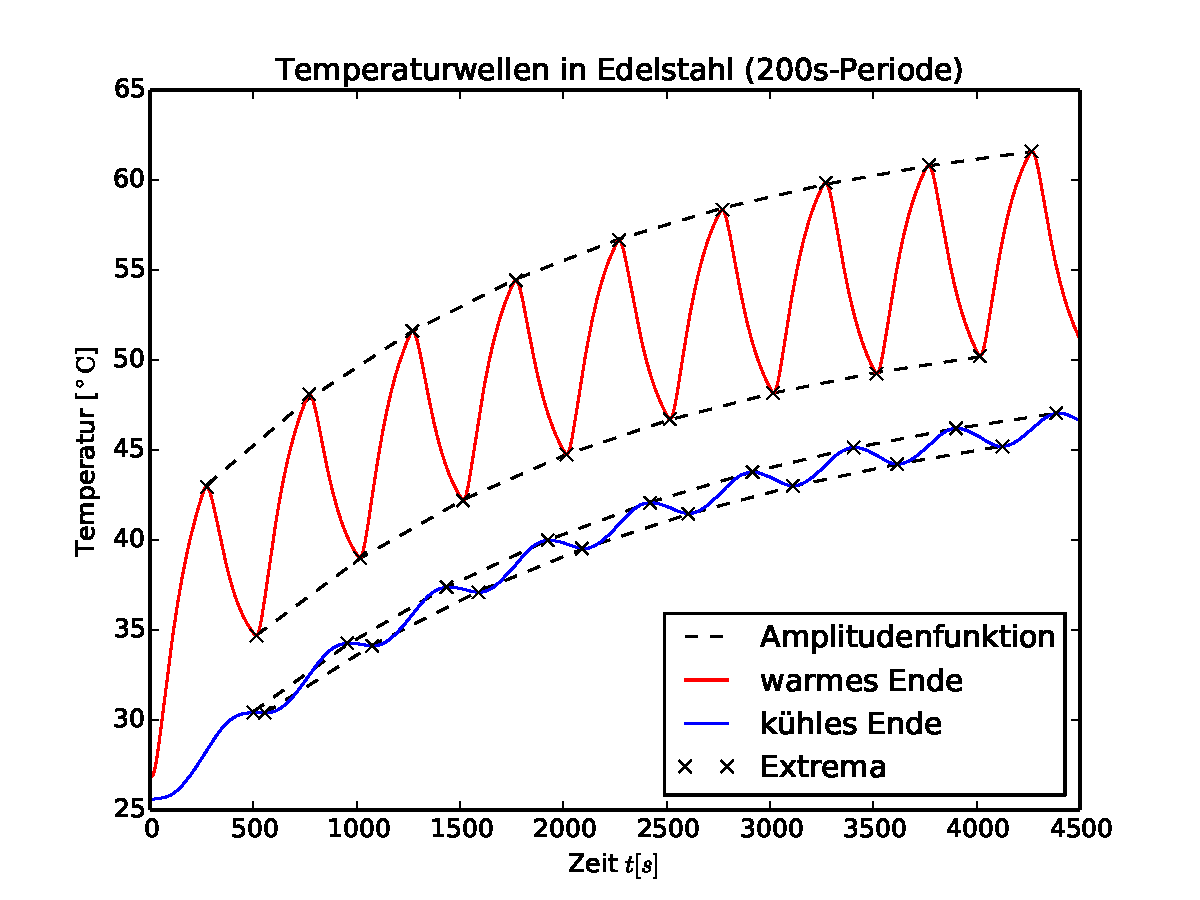
\includegraphics[width=\textwidth]{Bilder/M3_Edelstahl.pdf}
	\end{subfigure}
	\begin{subfigure}{0.9\textwidth}
	\centering
	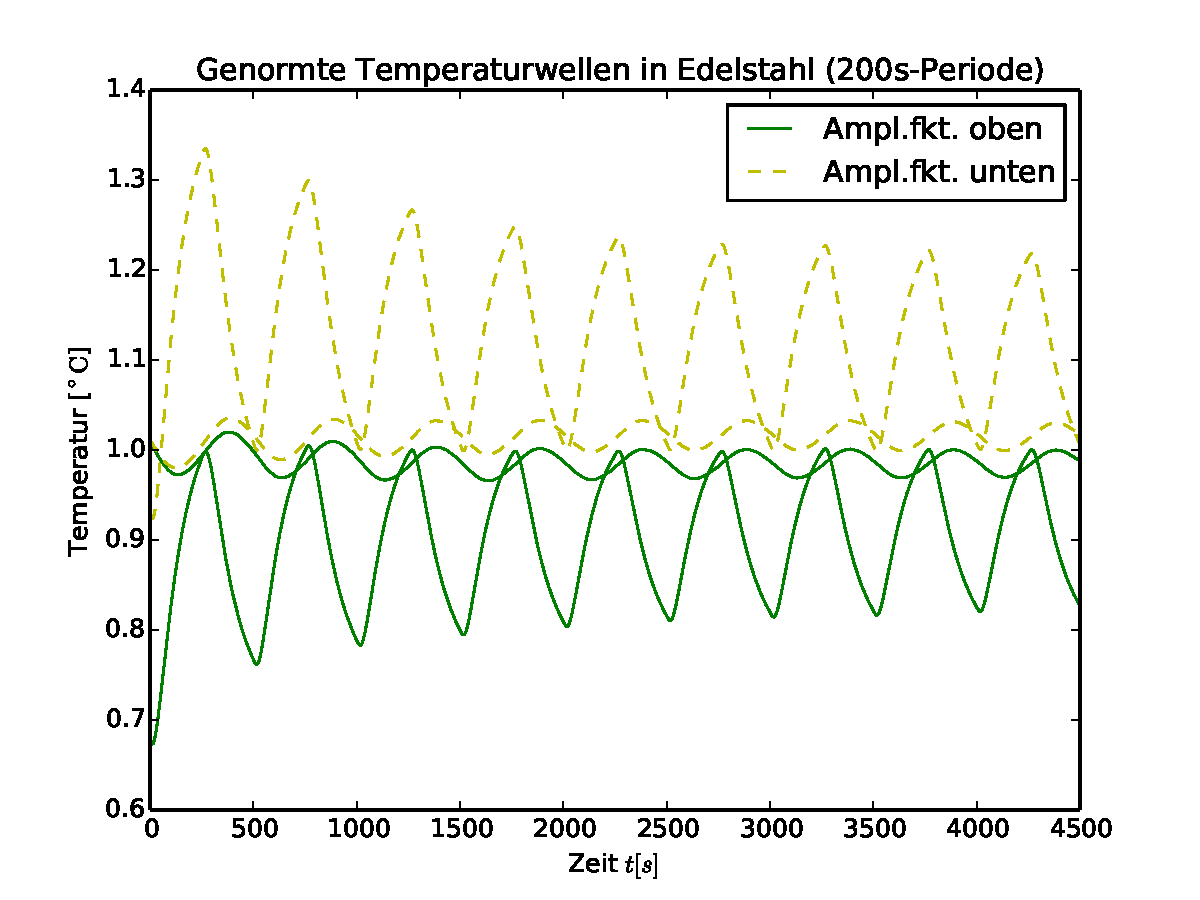
\includegraphics[width=\textwidth]{Bilder/Normierungsauswahl/M3_Edelstahl_norm.pdf}
	\end{subfigure}
	\caption{Periodische Messung bei Edelstahl mit 200 Sekunden-Periode sowie Eich-Möglichkeiten auf Grundschwingung}
	\label{fig:M3Edelstahl}
\end{figure}
\begin{figure}[h!]
	\centering
	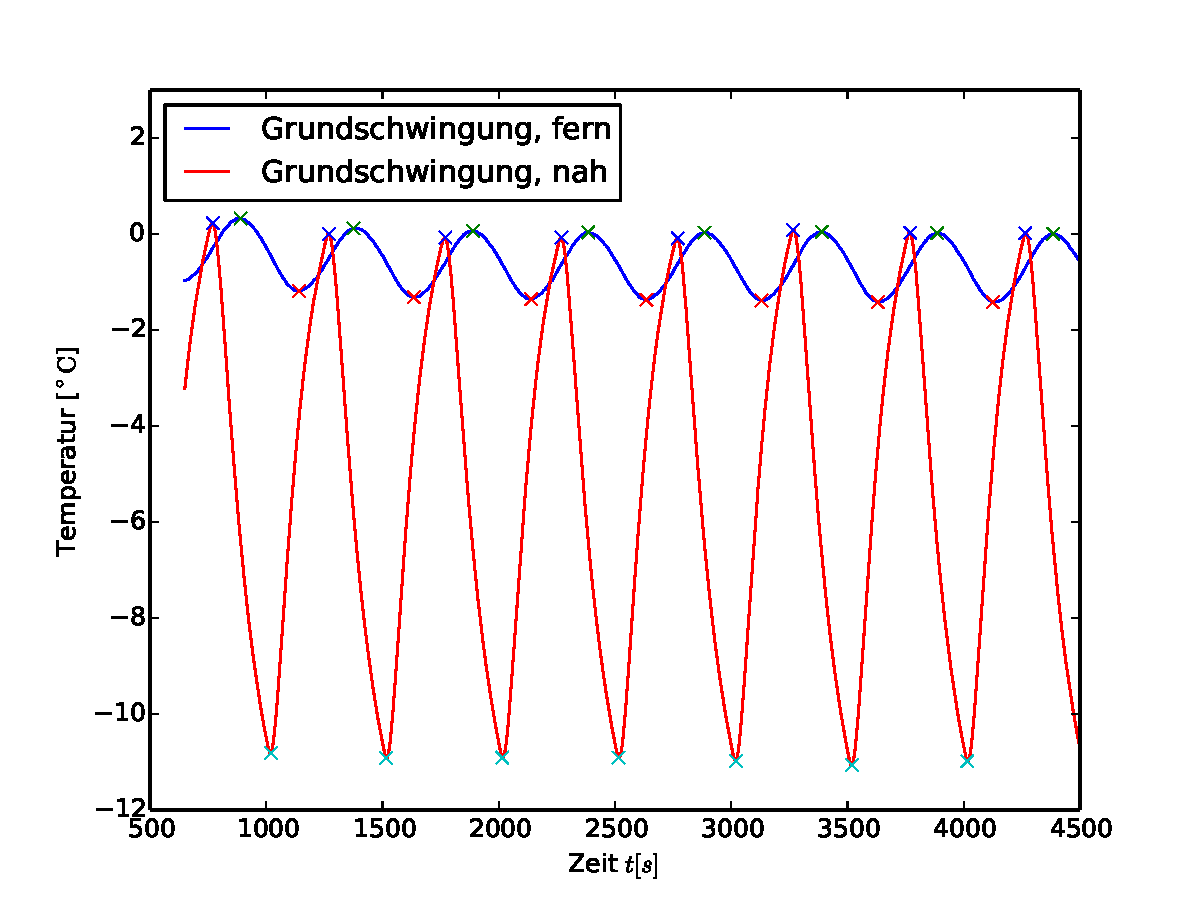
\includegraphics[width=0.7\textwidth]{Bilder/M3_Edelstahl_norm.pdf}
	\caption{Ausgewählter Teil der Grundschwingung von Edelstahl bei 200 Sekunden-Periode}
	\label{fig:M3EdelstahlNormkurve}
\end{figure}
\subsection{Bestimmung der Wärmekapazität}
Durch diese Grundschwingungskurven können die Amplituden $A_{\text{nah}}$ und $A_{\text{fern}}$ der Schwingung, sowie die Phasendifferenz $\Delta t$ zwischen den Messpunkten bestimmt werden; 
dabei wird der Teil der Grundschwingung vernachlässigt, der durch offensichtliche Verfahrensfehler mangelhaft ist
(vgl. Diagramme \ref{fig:M2Messing}, \ref{fig:M2Alu}).
Für die Amplitudenbestimmung werden in einem brauchbaren Abschnitt in der Grundschwingung Extremwerte bestimmt und die Mittelwerte der y-Koordinaten aller Maxima beziehungsweise Mimima errechnet.
Mit diesen Mittelwerten ist eine hinreichend genaue Beschreibung der Amplitude $A$ möglich.
Es gilt
\begin{equation}
	A = \frac{\bar{y}_{\text{Max}}-\bar{y}_{\text{Min}}}{2}.
\end{equation}
Für die Bestimmung der Phasendifferenz werden ausgezeichnete Punkte der Schwingung, hier Maxima, bestimmt und die Differenzen der x-Werte  gemittelt.
Es gilt
\begin{equation}
	\Delta{t_i} = {x}_{\text{Max, n+1}}-{x}_{\text{Max, n}}.
\end{equation}
\begin{table}[htbp]
	\centering
	\begin{tabular}{c S[table-format=1.5] S[table-format=1.5] S[table-format=3.3] c c}
		\toprule
		{Material}&{$A_\text{nah} \:/\si{\degreeCelsius}$}&{$A_\text{fern}\:/\si{\degreeCelsius}$}&{$\Delta{t}\:/\si{\second}$}&{$\rho$\:/\:\si{\kilo\gram\per\meter\cubed}}&{$c$\:/\:\si{\joule\per\meter\per\kelvin}}\\
		\midrule
		{Messing P2}& 	{3.1336}&{0.9034}&	{25.0}&		{8520}&{385}\\
		{Aluminium P2}&	{3.0011}&{1.5856}&	{18.75}&	{2800}&{830}\\
		{Edelstahl P3}&	{5.477}&{0.715}&	{116.875}&	{8000}&{400}\\
		\bottomrule
	\end{tabular}
	\caption{Kenngrößen der Grundschwingungen}
	\label{tab:kappazutaten}
\end{table}

Mithilfe der Amplituden $A_{\text{nah}}$ und $A_{\text{fern}}$, der Phasendifferenz $\Delta t$, der Geometrie und Beschaffenheit des Stabes kann mit der Gleichung \eqref{waermeleitfaehigkeit} die Wärmeleitfähigkeit $\kappa$ bestimmt werden.
\begin{table}[htbp]
	\centering
	\begin{tabular}{cccc}
	\toprule
	&\multicolumn{3}{c}{Wärmeleitfähigkeit \kappa \:/ \:\si{\watt\per\meter\per\kelvin}}\\
	&{Messing M2}&{Aluminium M2}&{Edelstahl M3}\\
	\midrule
	{Messung}&{47.4702}& 87.4175&6.0504\\
	{Literatur}&{120}&{236}&15\\
	\midrule
	{Abweichung}&60.44\%&62.96\%&59.6639\%\\
	\bottomrule
	\end{tabular}
	\caption{Wärmeleitfähigkeit $\kappa$ der Metalle.}
\label{tab:waermeleitfaehigkeitwerte}
\end{table}